%% Copyright (C) 2019-2021 Alessandro Clerici Lorenzini
%
% This work may be distributed and/or modified under the
% conditions of the LaTeX Project Public License, either version 1.3
% of this license or (at your option) any later version.
% The latest version of this license is in
%   http://www.latex-project.org/lppl.txt
% and version 1.3 or later is part of all distributions of LaTeX
% version 2005/12/01 or later.
%
% This work has the LPPL maintenance status `maintained'.
%
% The Current Maintainer of this work is Alessandro Clerici Lorenzini
%
% This work consists of the files listed in work.txt


\section{Serie}
Il calcolo delle serie (somme infinite) si pone il problema di calcolare espressioni come
\begin{gather}
	\label{serie:T}
	T=\sum_{k=0}^{+\infty}\frac{1}{2^k}=1+\frac{1}{2}+\frac{1}{4}+\frac{1}{8}+\frac{1}{16}+\dots\\
	\label{serie:W}
	W=\sum_{k=0}^{+\infty}(-1)^k=1-1+1-1+1-1+\dots\\
	\label{serie:V}
	V=\sum_{k=1}^{+\infty}\frac{1}{k}=1+\frac{1}{2}+\frac{1}{3}+\frac{1}{4}+\frac{1}{5}+\dots
\end{gather}
A questo scopo, si definisce la somma di una serie
\begin{defin}[Somma di una serie]
	Si definisce somma di una serie infinita il limite della somma parziale, per indice massimo che tende all'infinito:
	\[
		\sum_{k=0}^{+\infty} a_k:=\lim_{n\to+\infty}\sum_{k=0}^n a_k
	\]
	La somma parziale (o ridotta) si indica generalmente con $S_n$ e ha ordine $n$. Una serie si dice regolare se il suo limite esiste, convergente se è finito e divergente se è infinito.
\end{defin}

Quando una serie converge ne si valuta l'andamento (comportamento asintotico o $\Theta$) del resto, cioè la differenza tendente a zero tra la somma della serie e la somma parziale:
\begin{gather*}
	S_n\to S\in\R\\
	R_n=S-S_n\to0\\
	R_n=\sum_{k=0}^{+\infty}a_k-\sum_{k=0}^n a_k=\sum_{k=n+1}^{+\infty} a_k
\end{gather*}
Quando una serie diverge ne si valuta l'andamento della somma parziale, in quanto il resto è infinito:
\begin{gather*}
	S_n\to+\infty\\
	R_n=+\infty-S_n=+\infty\quad\forall n\in\N
\end{gather*}


\subsection{Serie geometriche}
Tornando all'esempio iniziale, le serie $T$ (\ref{serie:T}) e $W$ (\ref{serie:W}) sono casi particolari di una serie geometrica, di cui al paragrafo \ref{sum:geompar} si è valutata la somma parziale:
\[
	\sum_{k=0}^n x^k=
	\begin{cases}
		\frac{x^{n+1}-1}{n-1}\qquad & x\neq1 \\
		n+1\qquad                   & x=1
	\end{cases}
\]
Con per $x=\frac{1}{2}$ nel caso di $T$ e $x=-1$ nel caso di $W$. È semplice calcolare dunque i limiti delle somme parziali:
\begin{gather*}
	\text{per }n\to+\infty\\
	T=\sum_{k=0}^n \left(\frac{1}{2}\right)^k=\frac{\left(\frac{1}{2}\right)^{n+1}-1}{\frac{1}{2}-1}=2\left(1-\left(\frac{1}{2}\right)^{n+1}\right)\to2\\
	\text{con }R_n=S-S_n=\left(\frac{1}{2}\right)^n\\
	W=\sum_{k=0}^n (-1)^k=\frac{(-1)^{n+1}-1}{-1-1}=\frac{1-(-1)^{n+1}}{2}
\end{gather*}
Il secondo limite non esiste, per cui la serie non è regolare.

Si può generalizzare dicendo che
\begin{prop}
	Data una serie geometrica nella forma
	\[
		\sum_{k=0}^{+\infty} x^k
	\]
	\begin{itemize}
		\item essa converge se e solo se $\abs{x}<1$, e in tal caso vale
		      \begin{gather}
			      \sum_{k=0}^n x^k = \frac{x^{n+1}-1}{x-1}\to\frac{1}{1-x}=S\\
			      R_n=\sum_{k=n+1}^{+\infty} x^k=\sum_{j=0}^{+\infty} x^{j+n+1} = x^{n+1}\sum_{j=0}^{+\infty} x^j=\frac{x^{n+1}}{1-x}=\Theta(x^n)
		      \end{gather}
		\item essa diverge se e solo se $x\geq1$:
		      \[
			      S_n=
			      \begin{cases}
				      n+1\sim n\qquad                                                  & x=1 \\[1ex]
				      \dfrac{x^{n+1}-1}{x-1}\sim\dfrac{x^{n+1}}{x-1}=\Theta(x^n)\qquad & x>1
			      \end{cases}
		      \]
		\item la sua somma non esiste se $x\leq-1$
	\end{itemize}
\end{prop}

È da questa proprietà che deriva la razionalizzazione dei numeri con parte decimale periodica:
\begin{gather*}
	0,1\overline{27}=0,127272727\dots=\\
	=\frac{1}{10}+\frac{27}{1000}+\frac{27}{10^5}+\frac{27}{10^7}+\dots=\\
	=\frac{1}{10}+\frac{27}{10^3}\left(1+\frac{1}{10^2}+\frac{1}{10^4}+\frac{1}{10^6}+\dots\right)=\\
	=\frac{1}{10}+\frac{27}{10^3}\sum_{k=0}^{+\infty}\left(\frac{1}{10^2}\right)^k=\frac{1}{10}+\frac{27}{10^3}\left(\frac{1}{1-10^2}\right)=\frac{1}{10}+\frac{27}{10^3}*\frac{10}{99}
\end{gather*}


\subsection{Criterio del confronto integrale}
Il criterio del confronto integrale mira a stimare il comporamento di una serie tramite l'integrale di una funzione. Si consideri la seguente serie, chiamata serie armonica:
\[
	\sum_{k=1}^{+\infty}\frac{1}{k}
\]
Si consideri la funzione $y=\frac{1}{x}$, generalizzazione reale della successione della serie. Dal momento che l'obiettivo della procedura è quello di calcolare la somma tramite un'approssimazione integrale, si costruiscono delle aree uguali a $\frac{1}{k}$. Si faccia riferimento alla figura \ref{fig:intk}, in cui due aree di questo tipo, una approssimata per eccesso e una per difetto, sono costruite prendendo rettangoli di base unitaria e altezza $f(k)=\frac{1}{k}$.
\begin{figure}[ht]
	\centering
	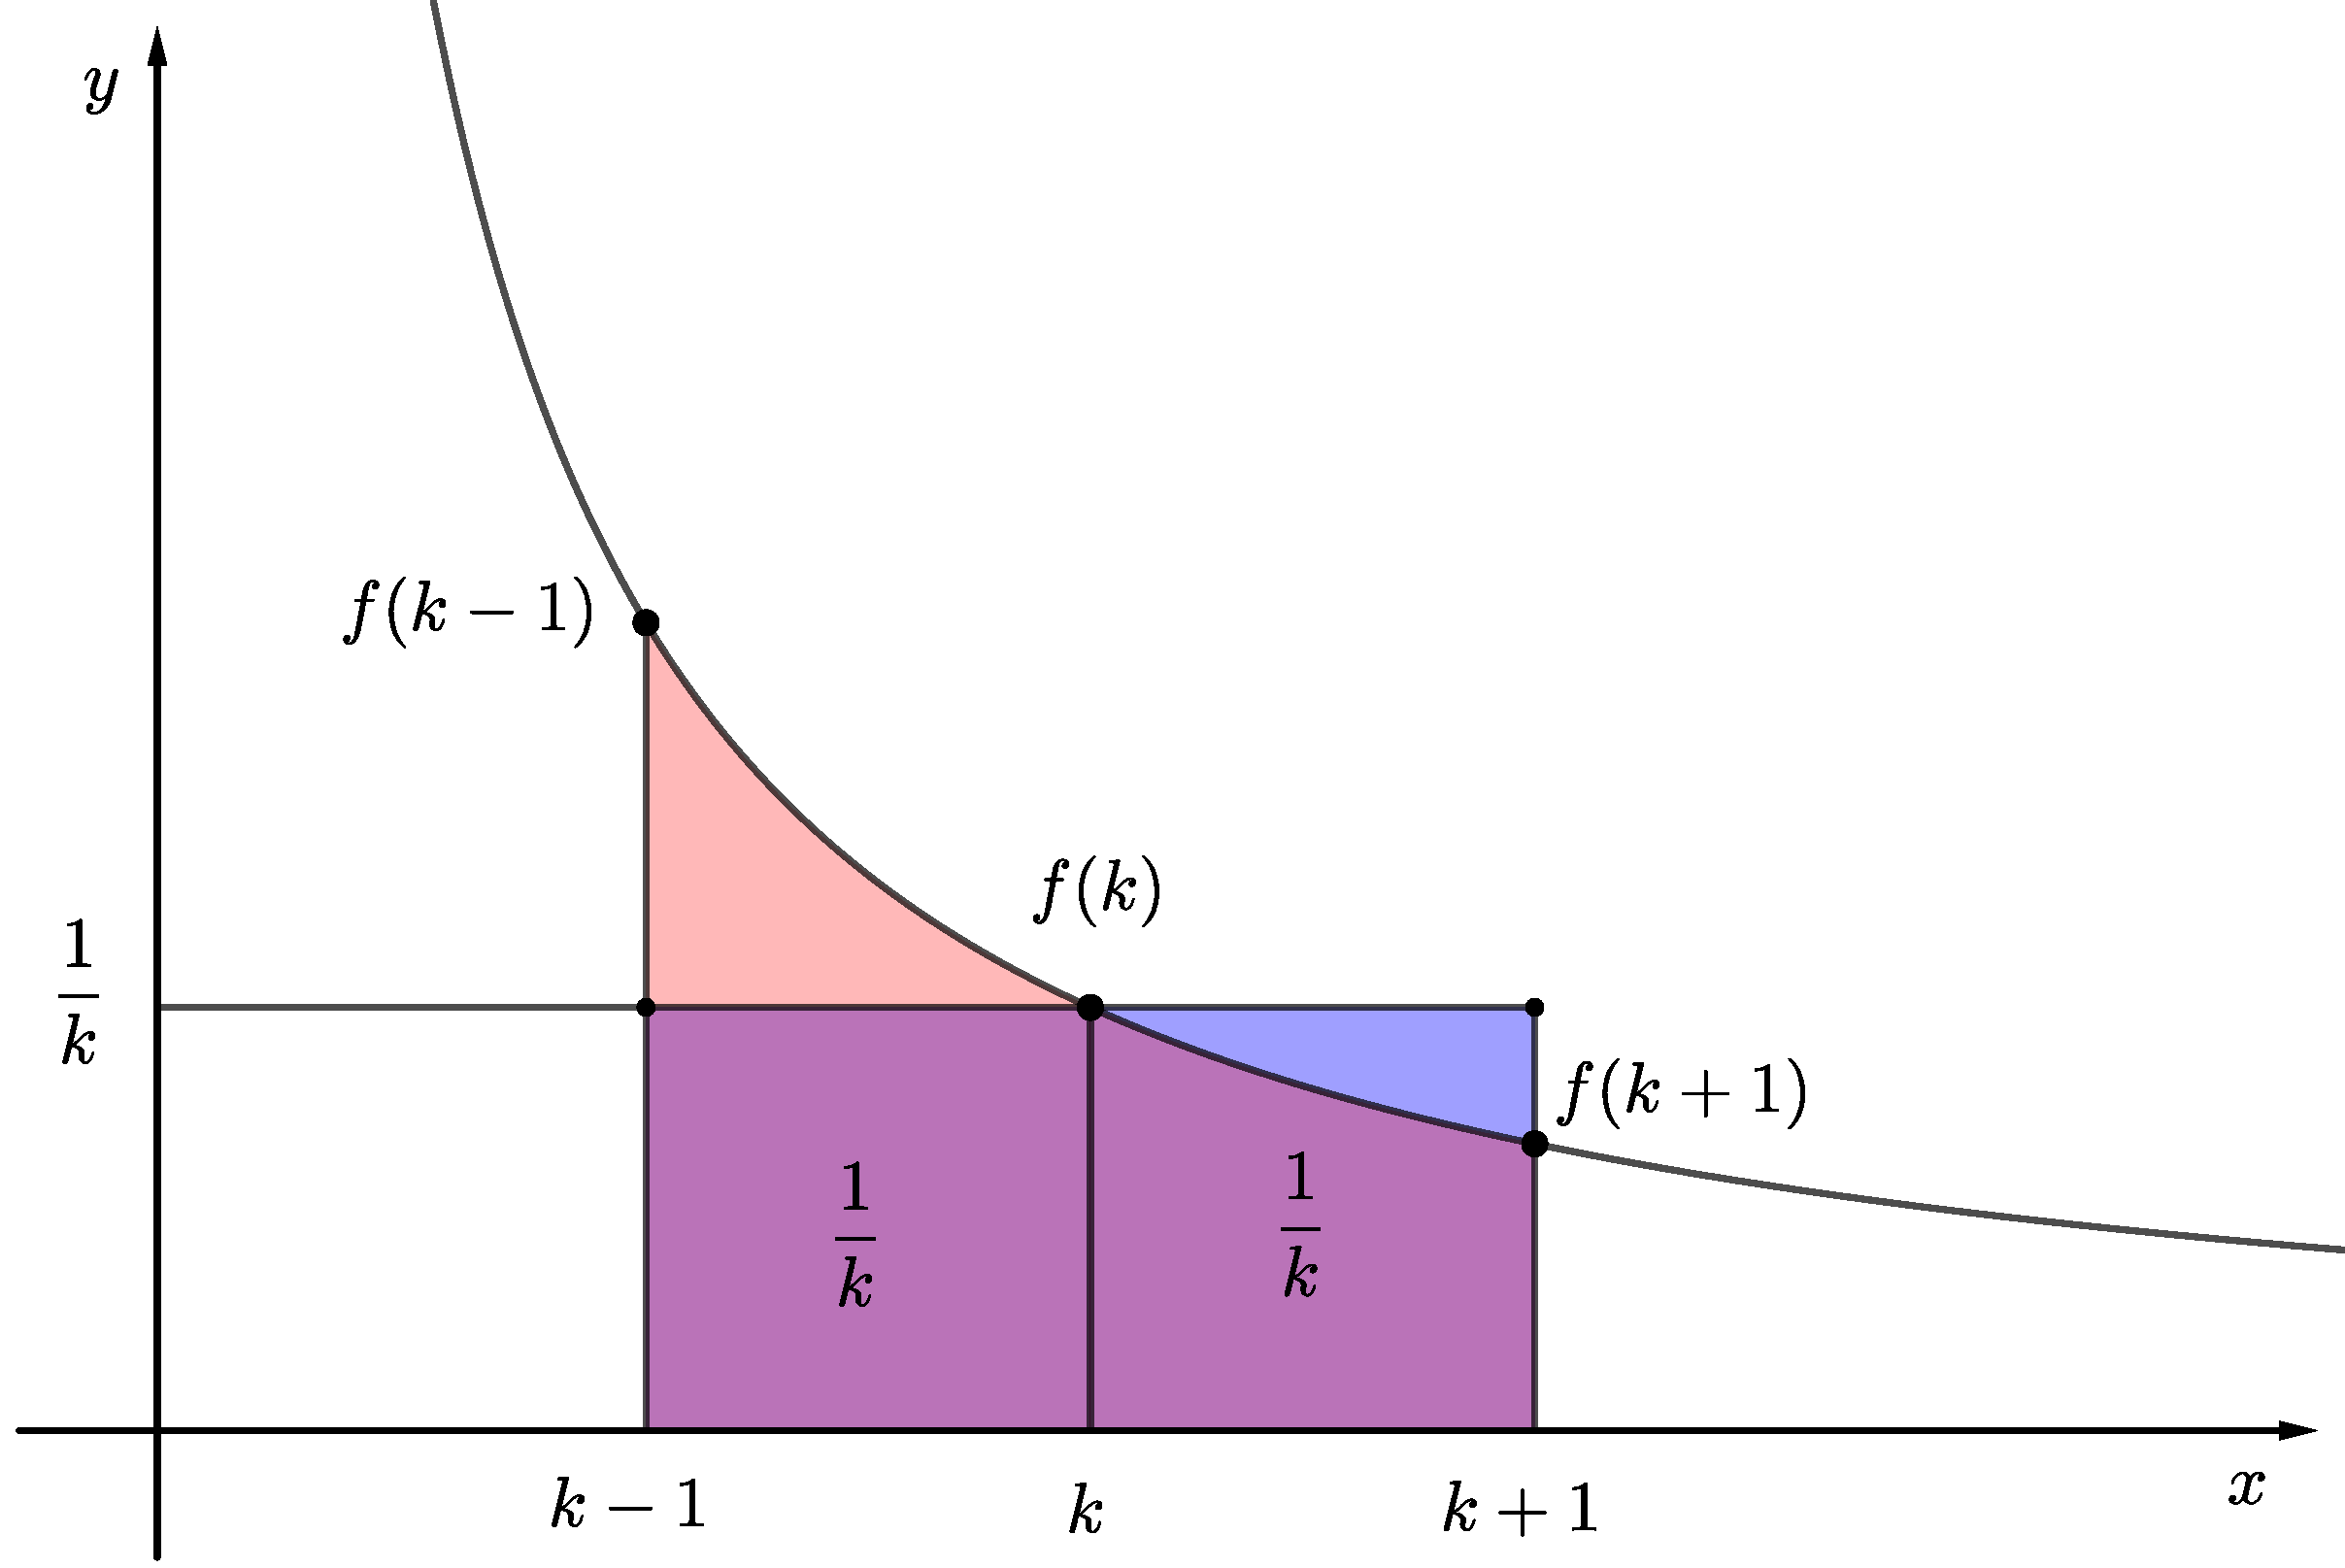
\includegraphics[width=0.7\textwidth]{grafici/intk}
	\caption{Approssimazione tramite integrale della somma della serie $\frac{1}{k}$.}
	\label{fig:intk}
\end{figure}
Da questa approssimazione si verifica che
\[
	\int_k^{k+1} \frac{dx}{x}\leq \frac{1}{k}\leq \int_{k-1}^k \frac{dx}{x}
\]
Estendendo l'approssimazione alla somma parziale:
\[
	\sum_{k=1}^n \int_k^{k+1} \frac{dx}{x}\leq \sum_{k=1}^n \frac{1}{k}\leq \sum_{k=1}^n \int_{k-1}^k \frac{dx}{x}
\]
Che applicando la proprietà \ref{int:somma} dell'integrale definito equivale a
\[
	\int_1^{n+1}\frac{dx}{x}\leq \sum_{k=1}^n \frac{1}{k} \leq \int_0^n\frac{dx}{x}
\]
Dalla prima disequazione si deduce che la somma parziale diverge, infatti:
\[
	\int_1^{n+1}\frac{dx}{x}=[\ln x]_1^{n+1}=\ln (n+1)\to+\infty
\]
Tuttavia, così com'è scritta la seconta disequazione non porta a nulla, dal momento che l'integrale improprio
\[
	\int_0^n\frac{dx}{x}=+\infty
\]
diverge in $0$ (infatti implica l'affermazione ovvia che la somma parziale sia minore di $+\infty$). È possibile però migliorare la stima: invece che stimare l'intero intervallo $(0,n)$ tramite l'integrale si utilizza per il primo valore della somma il valore stesso e per i successivi l'integrale:
\begin{align*}
	\sum_{k=1}^n \frac{1}{k} & \leq \sum_{k=1}^1 \frac{1}{k}+\int_1^n\frac{dx}{x} \\
	\sum_{k=1}^n \frac{1}{k} & \leq 1+\int_1^n\frac{dx}{x}
\end{align*}
Ovviamente, poiché come già dimostrato la somma parziale diverge anche la sua stima maggiore diverge:
\[
	1+\int_1^n\frac{dx}{x}=1+[\ln x]_1^n=1+\ln n
\]
Tuttavia, questo implica un'informazione ben più utile: poiché entrambi i valori di stima sono astintotici a $\ln n$, anche la somma parziale lo è:
\[
	\begin{cases}
		\ln(n+1)\sim \ln n \\
		1+\ln n\sim \ln n  \\
		\ln(n+1)\leq\sum_{k=1}^n \frac{1}{k}\leq 1+\ln n
	\end{cases}\Rightarrow
	\sum_{k=1}^n \frac{1}{k}\sim \ln n
\]

\begin{examp}
	Determinare il comportamento asintotico della seguente successione
	\[
		\ln(n!)
	\]
	La successione può essere espressa tramite una somma:
	\[
		\ln(n!)=\sum_{k=1}^n \ln k=\sum_{k=1}^n \ln k
	\]
	Questa somma può essere stimata tramite integrali della funzione $f(x)=\ln x$:
	\begin{gather*}
		\int_{k-1}^k \ln x ~dx\leq \ln k \leq \int_k^{k+1} \ln x ~dx\\
		\text{passando alle somme con $k=2$:}\\
		\int_1^n \ln x ~dx\leq \ln(n!) \leq \int_2^{n+1} \ln x ~dx
	\end{gather*}
	La primitiva di $f(x)$ è
	\[
		\int \ln x ~dx=x\ln x -\int x ~d(\ln x)=x\ln x -\int dx=x\ln x -x +c
	\]
	Quindi:
	\[
		n \ln n -n+1 \leq \ln(n!) \leq (n+1)\ln(n+1)-(n+1)-2\ln 2+2
	\]
	Entrambi i membri esterni sono astintotici a $n\ln n$, pertanto lo sarà anche la successione $\ln(n!)$.
\end{examp}

\begin{examp}
	Calcolare il limite di
	\[
		c_n=\sum_{k=n}^{2n} \frac{1}{k}
	\]
	Stimando tramite integrali ($f(x)=\frac{1}{k}$):
	\begin{gather*}
		\int_l^{k+1}\frac{dx}{x}\leq \frac{1}{k}\leq \int_{k-1}^k \frac{dx}{x}\\
		\int_n^{2n+1}\frac{dx}x \leq \sum_{n}^{2n} \frac{1}{k} \leq \int_{n-1}^{2n} \frac{dx}{x}\\
		\ln(2n+1)-\ln n \leq c_n \leq \ln(2n) -\ln(n-1)\\
		\ln\left(\frac{2n+1}{n}\right) \leq c_n \leq \ln\left(\frac{2n}{n-1}\right)
	\end{gather*}
	Essendo i membri esterni asintotici a $\ln 2$, il valore del limite è $\ln 2$.
\end{examp}

\begin{examp}
	Studiare il comportamento di
	\[
		\sum_{k=1}^{+\infty} ke^{-k}
	\]
	La serie si può stimare tramite integrali, tuttavia la funzione $f(x)=xe^{-x}$ non è elementare. Studiando la derivata $f'(x)=e^{-x}(1-x)$ si trova un unico massimo assoluto in $x=1$, dopo il quale la funzione decresce. Poiché per la stima integrale è necessaria una funzione monotona, si sceglie di partire da $k=2$, in modo che i rettangoli di base unitaria (si veda la figura \ref{fig:intk} riguardante però un'altra funzione non si estendano per $x<1$. Dal momento che la somma ha valori finiti per $k<2$ (uno), è possibile aggiungere tali valori "manualmente" dopo la stima. Per $k\geq2$ si ottiene:
	\begin{gather*}
		\int_k^{k+1} f(x)~dx \leq ke^{-k} \leq int_{k-1}^k f(x)~dx\\
		\int_2^{n+1} f(x)~dx \leq \sum_{k=2}^n ke^{-k} \leq \int_1^n f(x)~dx
	\end{gather*}
	L'integrale di $f(x)$ è
	\[
		\int xe^{-x}~dx=-\int x~d(e^{-x})=-xe^{-x}+\int e^{-x}~dx=-xe^{-x}-e^{-x}+c
	\]
	Tornando a $k\geq1$ e aggiungendo il valore della somma per $k=1$, ovvero $\frac{1}{e}$:
	\[
		\frac{1}{e}+\frac{3}{e^2} \leq \sum_{k=2}^n ke^{-k} \leq \frac{3}{e}
	\]
	Questa è una stima del valore della somma, che quindi converge. Per quanto riguarda lo studio del resto:
	\[
		\int_{n+1}^{+\infty} f(x)~dx \leq \sum_{k=2}^{+\infty} ke^{-k} \leq \int_n^{+\infty} f(x)~dx
	\]
	Svolgendo gli integrali impropri si ottiene:
	\[
		(n+2)e^{-(n+1)} \leq \sum_{k=2}^{+\infty} ke^{-k} \leq (n+1)e^{-n}
	\]
	Vale:
	\begin{gather*}
		(n+2)e^{-(n+1)}\sim ne^{-(n+1)}=\Theta(ne^{-n})\\
		(n+1)e^{-n}\sim ne^{-n}=\Theta(ne^{-n})
	\end{gather*}
	Quindi il resto è $\Theta(ne^{-n})$.
\end{examp}


\subsection{Proprietà delle somme finite nelle serie}
È innanzitutto utile menzionare la seguente proprietà
\begin{teor}[Condizione necessaria di convergenza]
	\label{teor:necconv}
	\[
		\sum_{k=0}^{+\infty} a_k\quad\text{converge}\quad\Rightarrow\quad a_k\to0\qquad k\to+\infty
	\]
\end{teor}
\begin{proof}
	\[
		\sum_{k=0}^n a_k-\sum_{k=0}^{n-1} a_k=a_n
	\]
	Le due somme non sono altro che successioni $S_n$ e $S_{n-1}$. Se per ipotesi $S_n\to S\in\R$, allora, per la proprietà delle successioni \vref{suc:trasl}, vale $S_{n-1}\to S$. La differenza di queste, cioè $a_n$, tende quindi a $0$.
\end{proof}

È naturale chiedersi se le proprietà applicate alle somme finite valgano anche per le serie infinite. La prima che è utile discutere è quella delle somme telescopiche (paragrafo \ref{sum:tele}). È possibile infatti applicare la proprietà alle somme parziali:
\[
	\sum_{k=1}^n a_k=\sum_{k=1}^n(b_k-b_{k+1})=b_1-b_{n+1}\to b_1-b_\infty
\]
Il limite della somma parziale, pertanto, esiste se
\[
	\exists \lim_{n\to+\infty} b_k := b_\infty
\]

Un'altra proprietà di cui ha senso questionare la validità è
\[
	\sum_{k=0}^{+\infty} a_k+b_k=\sum_{k=0}^{+\infty} a_k+\sum_{k=0}^{+\infty} b_k
\]
Da cui deriverebbe
\[
	\sum_{k=0}^{+\infty} c*a_k=c\sum_{k=0}^{+\infty} a_k
\]
Anche in questo caso ci si riconduce tramite la definizione alle somme parziali:
\[
	\sum_{k=0}^n (a_k+b_k)=\sum_{k=0}^n a_k + \sum_{k=0}^n b_k
\]
Posto che la prima somma sia regolare:
\[
	\exists \lim_{n\to+\infty} \sum_{k=0}^n a_k=a\qquad\land\qquad\exists \lim_{n\to+\infty} \sum_{k=0}^n b_k=b
\]
Che implica
\[
	\exists \lim_{n\to+\infty} \sum_{k=0}^n (a_k+b_k)=a+b
\]
A patto che i due limiti non siano infiniti discordi, nel qual caso si otterrebbe una forma di indecisione.


\subsection{Serie a termini definitivamente uguali}
\begin{teor}
	\label{ser:defugu}
	Se date due successioni $a_n$ e $b_n$ vale $a_n=b_n$ definitivamente, allora le relative somme infinite
	\[
		A=\sum_{n=0}^{+\infty} a_n, B=\sum_{n=0}^{+\infty} b_n
	\]
	hanno lo stesso carattere e la stessa velocità di convergenza/divergenza.
\end{teor}
\begin{proof}
	Per ipotesi:
	\[
		\exists\nu\mid a_n=b_n\forall n\geq\nu
	\]
	Dovendo calcolare il limite delle somme parziali per $n\to+\infty$, è lecito applicare ipotesi sulla grandezza arbitraria di $n$: in particolare, si pone $n\geq\nu$:
	\[
		A_n-A_{\nu-1}=\sum_{k=\nu}^n a_k=\sum_{k=\nu}^n b_k=B_n-B_{\nu-1}
	\]
	Da ciò si ricava che
	\[
		A_n=(A_{\nu-1}-B_{\nu-1})+B_n
	\]
	Ovvero, $A_n$ e $B_n$ differiscono di una costante $c_\nu$ dipendente solo da $\nu$. Questo significa che
	\[
		\lim_{n\to+\infty} A_n=c_\nu+\lim_{n\to+\infty} B_n
	\]
	Quindi:
	\begin{gather}
		A_n\to+\infty\Rightarrow B_n\to+\infty\land A_n\sim B_n\\
		A_n\to A\in\R\Rightarrow B_n\to B\in\R\land A_n\sim B_n
	\end{gather}
	E viceversa. Per quanto riguarda i resti, nel caso di convergenza:
	\[
		A-A_n=\sum_{k=n+1}^{+\infty} a_k=\sum_{k=n+1}^{+\infty} b_k=B-B_n
	\]
	Scelto $n\geq\nu$.
\end{proof}
Una conseguenza di questo teorema è che somme di serie di stesse successioni ma diversi indici minimi hanno lo stesso comportamento.

\subsection{Serie a termini definitivamente positivi}
\begin{teor}
	\label{ser:defpos}
	Se $a_k\geq0$ definitivamente, allora
	\[
		\sum_{k=0}^{+\infty} a_k
	\]
	è regolare.
\end{teor}
\begin{proof}
	La ridotta
	\[
		A_n=\sum_{k=0}^n a_k
	\]
	è definitivamente monotona crescente, infatti vale $A_{n+1}\geq A_n$ definitivamente poiché vale $A_{n+1}-A_n=a_{n+1}\geq 0$ definitivamente. Da ciò deriva che $A_n\to\text{sup}\{A_k\mid k\in\N\}$ (teorema \vref{suc:rego}), quindi la somma della serie esiste.
\end{proof}

\subsection{Criterio del confronto}
\begin{teor}[del confronto per le serie]
	\label{ser:confr}
	Date due successioni $a_k$ e $b_k$ a termini definitivamente positivi tali che $a_k\leq b_k$ definitivamente, se la serie che ha per termini le immagini di $b_k$ converge allora la serie che ha per termini le immagini di $a_k$ converge; se la seconda diverge allora la prima diverge. In simboli:
	\begin{gather*}
		\exists\nu\mid 0\leq a_k\leq b_k \quad\forall k\geq\nu\\
		\sum_{k=0}^{+\infty} a_k \text{ diverge}\quad\Rightarrow\quad \sum_{k=0}^{+\infty} b_k \text{ diverge}\\
		\sum_{k=0}^{+\infty} b_k \text{ converge}\quad\Rightarrow\quad \sum_{k=0}^{+\infty} a_k \text{ converge}
	\end{gather*}
\end{teor}
\begin{proof}
	Per $n\geq\nu$ (quindi opportunamente grande):
	\[
		\tilde A_n=\sum_{k=\nu}^n a_k\leq \tilde B_n=\sum_{k=\nu}^n b_k
	\]
	Se $\tilde A_n$ diverge si ha definitivamente
	\[
		M<\tilde A_n<\tilde B_n\qquad\forall M
	\]
	quindi $\tilde B_n$ è regolare e diverge. Essendo a termini definitivamente positivi, $\tilde A_n$ è regolare (teorema \ref{ser:defpos}). Se $\tilde B_n$ converge allora è limitata, quindi:
	\[
		\exists m \mid \tilde A_n \leq \tilde B_n\leq m
	\]
	Essendo $A_n$ limitata allora converge. Inoltre, essendo tali somme delle successioni, vale, per il teorema \vref{suc:glelandau}:
	\begin{equation}
		\tilde A_n =O(\tilde B_n)\quad\land\quad\tilde B_n =\Omega(\tilde A_n)
	\end{equation}
	e, nel caso di convergenza:
	\begin{equation}
		B-\tilde B_n=\Omega(A-\tilde A_n)\quad\land\quad\tilde A-A_n=O(B-\tilde B_n)
	\end{equation}

	Poiché definitivamente vale
	\[
		A_n=\sum_{k=0}^n a_k=\tilde A_n=\sum_{k=\nu}^n a_k\land B_n=\sum_{k=0}^n b_k=\tilde B_n=\sum_{k=\nu}^n b_k
	\]
	allora per il teorema \ref{ser:defugu} il comportamento delle somme iniziali è lo stesso.
\end{proof}
\begin{corol}
	\label{ser:confrasin}
	Date le serie degli $a_n$ e dei $b_n$ tali che $a_n,b_n\geq0$ definitivamente, vale
	\[
		a_n\sim b_n\quad\Rightarrow\quad \sum_{k=0}^n a_n=\Theta\sum_{k=0}^n b_n
	\]
	E le serie hanno, ovviamente, lo stesso carattere.
\end{corol}
\begin{proof}
	Poiché $\frac{b_n}{a_n}\to1$, si ha definitivamente:
	\[
		\frac{a_n}{2}\leq b_n\leq 2a_n
	\]
	Dal momento che le serie degli $\frac{a_n}{2}$ e dei $2a_n$ sono l'una $\Theta$ dell'altra, per il teorema \ref{ser:confr} la tesi è vera. Dimostrazione analoga occorre nel caso che come ipotesi si abbia $a_n=\Theta(b_n)$
\end{proof}

\begin{examp}
	Studiare la serie
	\[
		\sum_{k=1}^{+\infty}[1+2(k-\sqrt{k+k^2})]
	\]
	Sviluppando la radice con lo sviluppo notevole:
	\begin{gather*}
		1+2k\left(1-1-\frac{1}{2k}+\frac{1}{8k^2}+o\left(\frac{1}{k^2}\right)\right)=\\
		=1-1+\frac{1}{4k}+o\left(\frac{1}{k}\right)\sim\frac{1}{4k}=\Theta\left(\frac{1}{k}\right)
	\end{gather*}
	La serie diverge come $\ln n$ (serie armonica).
\end{examp}

\begin{examp}
	\[
		\sum_{k=2}^{+\infty}\frac{1}{(\ln k)^8}
	\]
	La serie è regolare dal momento che i suoi termini sono positivi. Inoltre, definitivamente vale:
	\begin{gather}
		\label{eq:serex1}
		1\leq(\ln k)^8\leq k\\
		\frac{1}{k}\leq\frac{1}{(\ln k)^8}\leq 1\notag
	\end{gather}
	Dalla la prima disequazione si deduce che la serie diverge. Per le somme parziali, applicando il teorema \ref{ser:confr}, vale inoltre:
	\[
		A_n=\Omega\left(\sum_{k=0}^n \frac{1}{k}\right)=\Omega(\ln n) \quad\land\quad A_n=O\left(\sum_{k=0}^n 1\right)=O(n)\\
	\]
	Volendo migliorare questa stima, si può notare che la seconda equazione della \ref{eq:serex1} vale anche per $k^\varepsilon$, $\forall\varepsilon>0$, da cui:
	\[
		A_n=\Omega(\ln n)\cap O(n^\varepsilon)
	\]
\end{examp}


\subsection{Convergenza assoluta}
\begin{defin}
	Si dice che una serie che ha per termini le immagini di una successione $a_n$ converge assolutamente se la serie che ha per termini le immagini di $\abs{a_n}$ converge:
	\[
		\sum_{k=m}^{+\infty} \abs{a_n}\to A\in\R
	\]
\end{defin}
\begin{teor}
	\label{teor:convass}
	Se una serie converge assolutamente, allora converge.
	\[
		\sum_{n=1}^{+\infty}\abs{a_n}\to A'\in\R\quad\Rightarrow\quad \sum_{n=1}^{+\infty} a_n\to A\in\R
	\]
\end{teor}
\begin{proof}
	Per ogni $a_n$ vale:
	\[
		-\abs{a_n}\leq a_n\leq \abs{a_n}
	\]
	Aggiungendo $a_n$ a tutti i membri
	\begin{gather*}
		\abs{a_n}-\abs{a_n}\leq a_n+\abs{a_n}\leq \abs{a_n}+\abs{a_n}\\
		0\leq a_n+\abs{a_n}\leq 2\abs{a_n}
	\end{gather*}
	Chiamando $b_n$ il membro centrale della relazione, si verifica che la serie che ha per termini le immagini di tale successione è convergente, dal momento che $b_n$ è maggiore di $0$ (da cui la regolarità) e minore di $2\abs{a_n}$, convergente per ipotesi. Dal momento che vale la relazione
	\[
		a_n\leq b_n-\abs{a_n}
	\]
	e le serie che hanno per argomento le due successioni al secondo membro convergono, allora anche $a_n$ converge.
\end{proof}


\subsection{Criteri della radice e del rapporto}
\begin{teor}
	Data una serie che ha per termini le immagini di una successione $a_n$ definitivamente non negativa, posto, se esiste:
	\begin{gather*}
		\sqrt[k]{a_k}\to L\\
		\frac{a_{k+1}}{a_k}\to L
	\end{gather*}
	\begin{itemize}
		\item Se $0\leq L<1$ allora la serie converge
		\item Se $L>1$ allora la serie diverge
	\end{itemize}
\end{teor}
\begin{proof}
	Si dimostra il criterio della radice. È possibile dimostrare il criterio del rapporto e che i due limiti $L$ sono uguali.

	In analogia con la dimostrazione del criterio della radice per le successioni (\vref{teor:sucradice}), per ogni coppia di estremi $p<q$ di un intorno di $L$ vale, definitivamente:
	\begin{gather}
		p<\sqrt[k]{a_k}<q\quad\Rightarrow\quad p^k<a_k<q^k\notag\\
		\label{eq:radiceserie}
		\sum_k^{+\infty}p^k<\sum_k^{+\infty}a_k<\sum_k^{+\infty}q^k
	\end{gather}
	\begin{itemize}
		\item Nel caso di $0\leq L<1$ è possibile scegliere un $q<1$. La serie dei $q^k$ sarà quindi una serie geometrica di ragione minore di $1$, pertanto converge. Per il teorema \ref{ser:confr} del confronto la serie degli $a_k$ converge;
		\item Nel caso di $L>1$ si ha $a_k>1$ definitivamente. Poiché la serie degli $a_k$ è regolare (essendo a termini definitivamente positivi) ma non soddisfa la condizione necessaria di convergenza (teorema \ref{teor:necconv}), la serie diverge.
	\end{itemize}
	In aggiunta alle conclusioni è possibile dire, per il teorema del confronto applicato alle serie della \ref{eq:radiceserie}, che
	\begin{itemize}
		\item Se la serie degli $a_k$ diverge:
		      \begin{gather*}
			      \sum^n a_k=\Omega\left(\sum^n p^k\right)\quad\land\quad \sum^n a_k=O\left(\sum^n q^k\right)\\
			      \sum^n p^k=\Theta(p^n)\quad\land\quad \sum^n q^k=\Theta(q^n)\\
			      \sum^n a_k=\Omega(p^n)\cap O(q^n) \qquad \forall(p<L<q)
		      \end{gather*}
		\item Se la serie degli $a_k$ converge, essendo
		      \[
			      R_n=S-\sum^n a_k=\Theta\left(\sum^n a_k\right)
		      \]
		      valgono le stesse considerazioni del caso precedente per $R_n$.
	\end{itemize}
\end{proof}
\begin{examp}
	\[
		\sum_{k=1}^{+\infty} \frac{k^2+2^k}{\ln k +\sqrt k}
	\]
	Vale
	\[
		a_k=\frac{k^2+2^k}{\ln k +\sqrt k}\sim \frac{2^k}{\sqrt k}=b_k
	\]
	Essendo la successione divergente, anche la serie lo è. Ai fini di studiare l'andamento, si applica il criterio del rapporto:
	\[
		\frac{b_{k+1}}{b_k}=\frac{2^{k+1}}{\sqrt{k+1}}*\frac{\sqrt k}{2^k}\to 2<1
	\]
	Da cui
	\[
		\sum_{k=0}^n b_k=\Omega(p^n)\cap O(q^n)
	\]
	Inoltre
	\[
		\frac{2^k}{\sqrt k}\leq 2^n\quad\Rightarrow\quad \sum_{k=0}^n b_k=\Omega(p^n)\cap O(2^n)
	\]
	Dal momento che, per il teorema \ref{ser:confrasin}, la somma parziale degli $a_k$ è $\Theta$ della somma parziale dei $b_k$, vi vale la stessa relazione, infatti:
	\[
		\sum_{k=0}^n a_k = \Theta\left(\sum_{k=1}^n\right)=
		\begin{cases}
			\Theta(\Omega(p^n))=\Omega(p^n) \\
			\Theta(O(2^n))=O(2^n)
		\end{cases}
	\]
\end{examp}
